
\begin{dialog}{六部无插入赋格}

\begin{quote}
阿基里斯带着大提琴来到螃蟹的住所,同螃蟹和乌龟一起举办一个室内乐晚会。主人螃蟹把他引进音乐厅,又走到门口去迎接他们共同的朋友乌龟。这间屋子里到处都是电子设备——各种完整的和破烂的唱机、连着许多键盘的电视屏幕,以及其他一些罕见的装置。在这些大功率的物件中间摆着一架普通的收音机。在这间屋子里的各种设备中,阿基里斯只知道到这台收音机怎么使,于是他走过去,有点鬼鬼祟祟地拧了拧收音机的调谐度盘。他调到了一个频道,里面有六个学者正在讨论自由意志和决定论的问题。他听了两句,然后带着点嘲弄的神情把它关上了。
\end{quote}

\begin{dialogue}

\item[阿基里斯]没有这种噪音我照样行。其实,对于想过这个问题的人来说,它挺清楚的,它就是——我是说,问题并不难解决,只要你理解了如何——或者,说得更抽象点,人们可以通过思考,或者至少想象某种情境来搞清全部情况,嗯,我本以为自己心里很明白这个问题。也许听听这个节目对我还是有好处的……

\dnote{(乌龟进来了,拿着他的小提琴。)}

嘿,嘿,小提琴家来了!你这个星期一直在练习吗,龟兄?我一天至少要练习两小时《音乐的奉献》中的三重奏鸣曲的大提琴部分,挺刻苦的吧?你知道,听音乐会的时候,你所听到的只是美妙动人的乐曲,可那是长期枯燥训练的结果,而那种翻来覆去的练习在别人听来简直就是噪音!

\item[乌龟]没有这种噪音我照样行。我发现偶尔练上一会儿就足以使我能很熟练地演奏了。

\item[阿基里斯]呃,你可真幸运啊。我要是也能这么轻松多好。哎。主人在哪儿啊?

\item[乌龟]我想他是取长笛去了。瞧,他来了。

\dnote{(螃蟹走进来,拿着他的笛子。)}

\item[阿基里斯]哦,老蟹,这个星期我一直在满怀热情地练习那首三重奏鸣曲,一边演奏我心里一边产生各种幻象:快活的咯咯叫的野蜂、忧郁的嗡嗡叫的火鸡,以及别的一些发着不同叫声的东西,音乐太具有魔力了!

\item[螃蟹]没有这种噪音我照样行。阿基,你不该把《音乐的奉献》当做是描写动物的作品。

\item[乌龟]老蟹说得对,阿基,《音乐的奉献》不是标题音乐。

\item[阿基里斯]不过,我喜欢动物,即使你们这两个迂夫子不赞成。

\item[螃蟹]我不认为我们是迂夫子,阿基。我们是说你听音乐有你自己的独特方式。

\item[乌龟]我们坐下来演奏吧。

\item[螃蟹]我期待着那位钢琴家朋友光临寒舍,为我们表演低音部。我亟愿您能与他一晤,阿基。然而他或不幸竟不能莅临。故我等不妨先开始,仅吾三人就足以演奏三重奏了。

\item[阿基里斯]老蟹,在我们开始以前,我想知道你摆在这儿的这么多各式各样的设备都是什么玩意儿?

\item[螃蟹]噢,它们大都是些零碎儿——破旧的唱机上的杂碎儿。是些纪念品\dlnote{(紧张地按着按钮)}——是使我出了名的那场龟蟹之战中留下来的。而那些连在电视屏幕上的键盘是我的新玩具。我一共有十五台,它们是新型的电子计算机,一种很小、很灵活的计算机——比起以前的计算机来要先进多了。很少有人像我这样对它们怀有如此之大的热情,然而我深信不疑:它们将来会很流行的。

\item[阿基里斯]它们有专门名称吗?

\item[螃蟹]有,它们叫“灵笨机”,因为它们非常有潜力,既能很机灵,又能很愚笨,全看操作者的技巧。

\item[阿基里斯]你是说你认为它们实际上可以变得——比如说——像人类那么机灵。

\item[螃蟹]可以这么说——因为,然唯有于灵笨机操作技巧训练有素者方能做得到。鄙人不曾有幸结识这方面的真正行家,甚是可惜。然邦外确有一专家,为众望所归——他若亲来,于不佞实为无上之欣悦,俾我亦可藉此有幸一睹灵笨机使用的真正技巧。然他竟未克惠临,致使吾几疑或竟无福享此乐趣。

\item[乌龟]跟一台由高手操作的灵笨机对弈一定十分有趣。

\item[螃蟹]此念甚妙。为灵笨机编一套高超的弈棋程序,会成为昭显技巧的极好标志。更为有趣的——然而也是复杂得令人难以置信的——是给一台灵笨机足够的指令,使它能胜任一场谈话。这会使人觉得它就是人!

\item[阿基里斯]这可太有意思了,我刚才还听了点关于自由意志和决定论的讨论呢,它又一次使我不得不思考这些问题。我承认,过去我想这些问题时,思想就很混乱,到最后我真的都不知道我在想什么了。可是这种有关一台可以跟你谈话的灵笨机的想法……它叫人莫名其妙。我是说,要是你就自由意志问题问问灵笨机的意见,它会怎么说呢?我还想,不知精于此理的你们二位愿不愿意按照你们对这个问题的理解给我解释解释,让我满足满足?

\item[螃蟹]阿基,你想象不出你的问题有多恰当。我谨愿我的琴师朋友在此,因为我知道你要是听到他在这一问题上的高论,一定会着迷的。趁他还不在,我想告诉你一段话,是我最近从一本书的结尾部分中一篇对话里看到的。

\item[阿基里斯]不是《金、银、铜——聚宝藏之精华》吧?

\item[螃蟹]不,我记得书名是《长颈鹿、大象、狒狒——热带草原的动物寓言》——或诸如此类的什么东西。反正是在刚才提到的那篇对话的结尾处,有个活宝引用了明斯基论自由意志的话。这之后不久,在跟另外两个人谈话时,那个活宝就音乐的即兴演奏问题又引了明斯基的话,还谈到Lisp语言、哥德尔定理。注意,他扯了这么一大堆,可根本没提明斯基!

\item[阿基里斯]啊,真不知耻!

\item[螃蟹]我应该承认,在那篇对话靠前的部分里,他暗示过他会在结尾处引用明斯基的话,所以这也许是可以原谅的。

\item[阿基里斯]我也有同感。不管怎么说,我很想听听明斯基对自由意志的高见。

\item[螃蟹]啊,是的……马尔文·明斯基说:“智能机一旦建立,如果发现它们在对心灵、意识、自由意志诸如此类事物上的信念同人一样混乱、一样固执,那将是不足为怪的。”

\item[阿基里斯]我喜欢这话!真是种有意思的想法。自动机认为自己有自由意志!这就像我认为我没有自由意志一样愚蠢!

\item[乌龟]我猜你也许没想到,阿基,我们三位——你、我、还有老蟹——可能是一篇对话里的三个角色,说不定那还是一篇跟老蟹刚才提到的相类似的对话呢。

\item[阿基里斯]哦,我当然想到了,每个正常人偶尔都会有这种想象。

\item[乌龟]还有食蚁兽、树懒、芝诺、甚至\emph{造物神}——我们可能全都是一本书里一系列对话中的角色哩。

\item[阿基里斯]的确有可能。作者说不定也会进来弹弹钢琴呢。

\item[螃蟹]此亦吾所愿也。然他素来迟到。

\item[阿基里斯]你还真认为我信以为真啦!我可知道我没有被另外什么有智慧的生物以任何方式控制!我的思想是我自己的,我按照我的愿望来表达——这点你不能否认!

\item[乌龟]这些谁也没否认,阿基。但是你所说的一切同你在某篇对话里所担任的角色是极为一致的。

\item[螃蟹]那篇文章——

\item[阿基里斯]我反对!也许老蟹的那篇文章和我的反对都被机械地决定了,可我拒绝相信这种说法。我可以接受物理决定论,但是我不能接受我只不过是某种别的智慧生物的虚构物的想法!

\item[乌龟]你是不是有个硬件的大脑这确实不重要,阿基,如果你的大脑是别人大脑中软件的一部分,你的意志同样是自由的。而他的大脑说不定也是某种更高层次的大脑中软件的一部分……

\item[阿基里斯]多荒诞的想法!不过,我得承认,我确实愿意去找找那些巧妙地隐藏在你诡辩里的漏洞,来吧,争取说服我,咱们较量较量。

\item[乌龟]你没注意到吗,阿基,你的朋友们都有点不同一般?

\item[阿基里斯]当然。你很古怪(我知道我说这话你不在意),甚至老蟹也有点怪怪的(原谅我,老蟹)。

\item[螃蟹]哦,不必多虑。

\item[乌龟]可是,阿基,你忽视了你的朋友们的一个最显著的特征。

\item[阿基里斯]哪个特……?

\item[乌龟]我们都是动物啊!

\item[阿基里斯]哦,哦——是这样。你们个个儿都这么聪明。你要是不说,我还真不会这么明晰地意识到这一事实呢。

\item[乌龟]这还不是充分的证据吗?就你所知,有多少人成天同会说话的乌龟、螃蟹呆在一起?

\item[阿基里斯]我得承认,一只会说话的螃蟹是——

\item[螃蟹]当然是挺反常的。

\item[阿基里斯]没错儿,是反常——不过这是有先例的,文学作品里有过这种事。

\item[乌龟]对——文学作品里有,可现实生活里有吗?

\item[阿基里斯]叫你这么一说,我还真回答不上来了。我得想想。不过,这还不足以使我相信我是一篇对话中的一个角色。你有别的证据吗?

\item[乌龟]你还记得有一天我们在公园里相遇了,而且从表面上看纯属偶然?

\item[阿基里斯]是我们讨论艾舍尔和巴赫的《螃蟹卡农》的那天吗?

\item[乌龟]正是!

\item[阿基里斯]还有老蟹,我想起来了,他在我们的谈话进行到近一半时不知从哪儿冒了出来,唠叨了一些怪事,然后又离开了。

\item[螃蟹]不是“近一半时”,阿基,是恰好一半时。

\item[阿基里斯]嗯,就算是吧。

\item[乌龟]你发现没有,谈话中你说的话跟我说的是一样的——只是顺序相反?只有个别词改动了,但总的来说,我们那次相遇有一种时间对称。

\item[阿基里斯]那有什么!那不过是变戏法。也许都是用镜子变出来的。

\item[乌龟]不是什么戏法,阿基,也没有镜子:这正是那位勤奋的作者的功劳。

\item[阿基里斯]哦,我觉得谈这个真没劲。

\item[乌龟]怎么回事,你常常觉得没劲儿吗?

\item[阿基里斯]哎,这段话我觉得挺熟,好像在哪儿听到过类似的话,可我忘了是谁说的。

\item[乌龟]你说的,阿基。

\item[螃蟹]这些话也许那天在公园说过,阿基。你还能回忆起那天你跟龟兄的谈话是如何进行的吗?

\item[阿基里斯]模模糊糊。开头他说:“周末愉快,阿基”,而结尾时,我说:“周末愉快,龟兄”,对吗?

\item[螃蟹]我这儿正好有个抄本……

\dnote{(他在他的音乐箱里摸来摸去,抽出一张纸条,递给阿基里斯。随后一边留心阿基里斯,一边烦躁不安地动来动去。)}

\item[阿基里斯]这真怪,非常非常奇怪……就是在一瞬间,我察觉到了某种——古怪。好像有人实际上事先安排好了全套对话,甚至连我那天谈话中的每个细节都计划好了。也就是说,原来我们一直是在那个人的大脑里吵吵嚷嚷,天呐,这得是多大的噪音啊!必须经过这样一个阶段才能把这一切写出来吗?

\dnote{(这时,门突然打开了,作者走进来,拿着一大摞手稿。)}

\item[作者]没这种噪音我照样行。你们知道,我的角色一旦形成,它们似乎就有了自己的生命,安排它们的对话我不用费多大劲儿。

\item[螃蟹]嘿,你来了!我还以为你不来了呢。

\item[作者]很抱歉来晚了。我走差了道儿,还岔得挺远。不过,我还是回来了。再次见到你们很高兴,龟兄、老蟹。阿基,见到你我特别高兴。

\item[阿基里斯]你是谁?我以前从没见过你。

\item[作者]我是侯世达——叫我老侯好了——我现在正在写一本书,书名是《哥德尔、艾舍尔、巴赫——集异璧之大成》。你们三位都是这本书里的角色。

\item[阿基里斯]见到你很愉快。我的名字是阿基里斯,而——

\item[作者]无需介绍你自己,阿基,我已经熟知你了。

\item[阿基里斯]奇怪,奇怪。

\item[螃蟹]他就是我说要来为我们演奏钢琴的那位先生。

\item[作者]我在家里已经用钢琴弹了一点《音乐的奉献》,总是不能完全不出错儿。要是你们能迁就的话,我可以凑合着弹弹那首三重奏鸣曲。

\item[乌龟]哦,我们这里的人都挺宽容的,都是业余爱好者嘛!

\item[作者]我希望你不在意,阿基,我想那天你跟龟兄在公园里说了顺序相反的相同的话,这事儿得怪我。

\item[螃蟹]别忘了我!我也在那儿,在谈话时,我也扯了一会儿呢!

\item[作者]当然!你是《螃蟹卡农》里的那只螃蟹。

\item[阿基里斯]所以你说是你操纵了我们的谈话?我的大脑是你大脑中的软件子系统?

\item[作者]你想这么说也可以,阿基。

\item[阿基里斯]设想我写了些对话,那谁算是这些对话的作者呢?你还是我?

\item[作者]当然是你啦。至少在你所在的那个虚构的世界里,你被认为是作者。

\item[阿基里斯]虚构的?我看不出它是虚构的!

\item[作者]而我也会在我所在的世界里被认为是作者,虽然我还不能肯定这样做对不对。而那个使我让你写下你的对话的人会在他的世界里被认为是作者(从他那里看,我的世界就是虚构的了)。

\item[阿基里斯]太叫人不敢相信了。我以前从未想到我的世界之上还有一个世界——而现在你暗示在这之上有一个。这就像爬一段熟悉的楼梯一样,在你走到头儿之后还要往上走——或者说,在你走完通常已走到头儿的一段之后,还要继续上。

\item[螃蟹]换句话说,从你过去认为是现实的生活中醒来,发现它乃幻梦而已。这可以一再发生,无法逆料它会止于何时。

\item[阿基里斯]最叫人困惑的是我梦中的人物怎么会有它们自己的意志,怎么能独立于我的意志而各行其是。仿佛在我做梦的时候,我的心智只是个舞台,在它上面某些别的有机体具有了自己的生命。而当我醒来时,它们就都溜掉了。我真想知道它们到哪儿去了……

\item[作者]你把它们赶走时,它们就都跑到嗝所去的地方了:到堕界去了。打出的嗝和梦中的生命都是一些软件子有机体,存在于外在宿主有机体中。宿主有机体为它们提供了舞台——或者甚至可以说提供了宇宙。一时间它们具有了生命,但是若宿主有机体的状态发生了变化——例如,醒来——那么,那些子有机体就瓦解了,不再作为彼此独立、自身统一的东西而存在了。

\item[阿基里斯]就像沙堡,一个浪头打来,便会消失得无影无踪,是吗?

\item[作者]正是这样。嗝、梦中的人物,甚至对话中的角色,当它们的宿主有机体发生某种状态变化时,就会统统瓦解。然而,正像你描述的那些沙堡一样,所有形成它们的那些东西依然存在。

\item[阿基里斯]我反对只是像个嗝那样存在!

\item[作者]可我现在也要把你比作沙堡,阿基。这不很有诗意吗?此外,要是你只不过是我大脑里的一个嗝,那我也不过是某个层次的作者大脑里的一个嗝,这一事实也许会给你些安慰。

\item[阿基里斯]可我是这么一个活生生的生物啊——很显然是由血肉和骨头构成的。这你不能否认!

\item[作者]我无法否认你的这种感觉,可是想想梦中的生物吧:虽然他们不过是软件的幽灵,却具有一点不比你少的相同感觉。

\item[乌龟]哎,我说,够了,够了!让我们坐下来演奏吧!

\item[螃蟹]主意甚佳——且现有作者惠临,他会以其对三重奏鸣曲之钢琴部的演奏愉悦我等之耳的,此作曾被巴赫弟子科恩伯格加过和声。幸哉我等!\dlnote{(领作者到他的一架钢琴前)}我希望您觉得座位舒适,您可以调调位置,您——\dlnote{(屋子里响起奇怪而柔和的振动声。)}

\item[乌龟]请原谅,这奇怪的电子声是怎么回事?

\item[螃蟹]啊,此乃发自一灵笨机,意为将有新通知闪过屏幕。此类通知常只是些来自控制着所有灵笨机的主控程序的不太重要的通告。\dlnote{(他手里拿着长笛走到灵笨机前,看着它的屏幕,随即兴奋地转向聚在一起的乐师们)}先生们,老巴来了。\dlnote{(他把长笛放到一边)}我们理当马上迎迓他进来。

\item[阿基里斯]老巴!是那个你选来今晚在此给我们表演的著名即兴演奏家吗?

\item[乌龟]老巴!这只能是指一个人——那个著名的查尔斯·巴比奇先生,文学士、皇家学会会员、皇家工程学会会员、皇家天文学会会员、皇家统计学会会员、皇家艺术学院荣誉院士、帝国道德学院成员、皇家白俄经济学会会员、摩纳哥皇家学院院士、彼得堡帝国和皇家学院院士、意大利圣莫里斯和圣拉撒路协会会长、美国波士顿科学与艺术学院院士、日内瓦国家物理学及历史学学会会员、提取器俱乐部成员、等等等等。巴比奇是计算技巧和计算科学的最受尊敬的开拓者。多么珍贵的荣誉啊!

\item[螃蟹]他遐迩闻名,我素来期望他屈尊惠至——这可是完全出人意料的。

\item[阿基里斯]他也演奏乐器吗?

\item[螃蟹]素闻他于近百年里嗜印度手鼓、口哨及种种其它巷闾乐器,颇令人不解。

\item[阿基里斯]这么说,他也许会加入我们的音乐晚会呢。

\item[作者]我建议我们为他行十响卡农礼。

\item[乌龟]演奏《音乐的奉献》中所有著名的卡农曲?

\item[作者]没错儿。

\item[螃蟹]妙啊!快,阿基,请依演奏顺序列出十首,他一进来就交给他!然鄙人担心彼或以吾辈以业余爱好者之水平演奏此曲,几同噪音。

\dnote{(阿基里斯还没动地方,巴比奇就进来了。他拿着一把手摇风琴,穿着一件笨重的旅行外套,戴着帽子。他因长途旅行而显得有点疲倦和衣冠不整。)}

\item[巴比奇]没有这种噪音我照样行。\emph{无}需\emph{插入}这种仪式,贵府就已经\emph{赋}有丰富的艺术\emph{格}调了。

\item[螃蟹]巴先生!十分高兴您光临“坦茨波”,使蓬筚生辉。多年来我一直翘望与您结识,今日终得如愿。

\item[巴比奇]哦,蟹先生,我敢说这种荣幸实属不佞:有幸见到您这样一位在所有学科都如此声名蜚然的名士、一位具备令人不可企及的音乐知识和技巧的大师、一位如此好客逾常的东道主。我还敢说您对您的客人的衣着也一定要求很高,然而我必须承认我无法满足这些最合理的要求,但无论如何,衣着亵慢不适合您这位如此著名和优秀的螃蟹臂下之访客的身份。

\item[螃蟹]如果我理解了您这最值得赞美的自白,最受欢迎的客人,我臆度您是倾向于改换一下您的装束的。我向您保证,对于今晚这种环境来说,再没有什么服装比您的更合适了。请您卸装吧,而且,要是您对这些水平不高的爱好者的音乐演出不反感,就请接受由塞巴斯第安·巴赫的《音乐的奉献》中的十首卡农组成的一份“音乐的奉献”,以此表达我们的仰慕之情。

\item[巴比奇]受到您超级热情的接待,使我愉快得十分手足无措,蟹先生。我要最谦谨地回答说,我无法表达更深的谢意,以感谢你们将为我举行的卓越的老巴赫的音乐演奏会,他作为一个管风琴家和作曲家是盖世无双的。

\item[螃蟹]啊不!我还有个更好的主意,相信它也会得到我最尊敬的客人的赞同。这个主意是,给您一个机会,巴先生,作为第一个试用“灵笨机”的人。这是我新近弄到,但尚未检验过的一种新意儿——一种分析机的现代实现,如果您愿意接受这种说法的话。您作为一个计算机的程序设计名家早已闻名遐迩,僻远如坦茨波也传颂着您的大名。对我们来说,观看您驾驭这种新型的战无不胜的灵笨机的技巧是一种无上的乐趣。

\item[巴比奇]久未耳聆这样杰出的想法了。愿意满足试用您的新型灵笨机的要求,我迄今只是耳闻了一些有关它的情况。

\item[螃蟹]让我们开始把!但是请原谅我的疏忽!我早应该向您介绍我的朋友们了。这是乌龟先生,这是阿基里斯,这是作者侯世达。

\item[巴比奇]有幸与你们结识,我感到非常愉快。\dlnote{(人们都走到灵笨机前,巴比奇坐下来,手指掠过键盘。)}手感很舒适。

\item[螃蟹]您喜欢它我很高兴。

\dnote{(突然,巴比奇指法优美而熟练地按动键盘,输入了一个又一个指令。几秒钟后,他停下来,几乎同时,屏幕上开始出现数字。刹那间,屏幕上满是数以千计的小个数字,最前面的几个是:$3.14159265358979323846264\ldots$)}

\item[阿基里斯]$\uppi$!

\item[螃蟹]多精巧啊!我从未想到用这么简单的算法能这么快地算出这么多位数!

\item[巴比奇]功劳完全属于灵笨机。我的作用只是了解它里面潜在地有什么,并用适当有效的方法利用它的指令集。真的,任何人只要实践过都能掌握这种技巧。

\item[乌龟]您可以作图吗?

\item[巴比奇]我可以试试。

\item[螃蟹]妙极了!让我带您到另一架灵笨机这儿来吧。我想请您都试试!

\dnote{(于是巴比奇被领到另一架灵笨机前坐下。他的手指又一次敲击着灵笨机的键盘,只一瞬间,屏幕上就出现了无数摇动着的线条。)}

\item[螃蟹]这些旋起的图形,在它们不断地彼此冲撞和干扰时,有多么和谐、动人啊!

\item[作者]它们从不完全重复,甚至从不跟以前出现过的相像。它的美看去似乎具有无可穷尽的层次。

\item[乌龟]一些是简单而悦目的图形,另一些则是令人迷乱同时也是令人爽心的复杂得难以描述的旋圈。

\item[螃蟹]您看出来了吗,巴先生,屏幕是彩色的?

\item[巴比奇]哦,真的吗?这样我就可以用这种算法做更多的花样了。只消一会儿。\dlnote{(键入一些新的指令,并马上按下两个键。)}当我松开的时候,所有的色彩都会显示出来\dlnote{(松开键)}。

\item[阿基里斯]哦!多富丽的色彩!有些图形一看就像要跳出来似的。

\item[乌龟]我认为那是因为它们的形状都在增大。

\item[巴比奇]那是有意的,图形增大,愿您螃蟹臂下的运气也增大。

\item[螃蟹]谢谢您,巴先生,任何言辞也无法表达我对您操作的欣赏!您在我的灵笨机上的操作是前所未有的。嘿,您摆弄灵笨机就好像它们是乐器,巴先生!

\item[巴比奇]恐怕我能奏出的任何音乐在您这样一位高贵的螃蟹臂下听来都太嘈杂了。虽然我近年来倾心于手摇风琴那甜美的声音,可我还是很清楚别人听它们时那种刺耳的效果。

\item[螃蟹]不管怎么说,接着试灵笨机吧!事实上我有一个新想法——一个不可思议的令人激动的想法!

\item[巴比奇]什么想法?

\item[螃蟹]我最近创作了一个主题,我这会儿突然想到,在所有的人当中,您巴先生是最适合使我那潜在主题成为现实的人!你们是否都熟悉哲学家拉·梅特利的思想?

\item[巴比奇]名字听起来很熟,请提示一下。

\item[螃蟹]他是位唯物主义的斗士。1747年,他在腓德烈大帝的宫廷里写了一本名叫《人是机器》的书。在这本书里面,他说人如同一架机器,尤其是人的智能。我的主题来自他这一论点反过来的思考:使一架机器中充满了人的心智机能——比如说理解力——会怎么样?

\item[巴比奇]我时时虑及这类问题,只是从未有合适的硬件材料来处理它们。这确是一绝妙建议,蟹先生,依照您的主题进行工作我会感到无比快乐的。告诉我——您心里已经有了关于某种智能的想法了吗?

\item[螃蟹]偶然有过一个想法:即指导它下一手漂亮的国际象棋。

\item[巴比奇]多新颖的建议!国际象棋正好是我最喜欢的消遣。我得说您对计算机器有广博的知识,绝不仅仅是个业余爱好者。

\item[螃蟹]事实上,我所知甚少。我的贡献只不过是我似乎能创造一些主题,而发挥这些主题的潜能非吾力所能及。这个主题是我最喜欢的。

\item[巴比奇]我非常愿意竭尽愚诚实现关于教灵笨机下国际象棋的设想。毕竟,服从您臂下的意旨乃我辈之职分。\dlnote{(他一边这样说着,一边转移到另一台灵笨机前,开始敲起来。)}

\item[阿基里斯]嘿,他的手移动得多娴熟,就好像在演奏音乐。

\item[巴比奇]\dlnote{(用一种特别优美的装饰性指法来结束他的表演)}当然,我确实还没有什么机会来证明灵笨机的下棋能力完全无可挑剔,不过也许这会使您至少可以验证一下跟灵笨机下棋的设想的可行性,即使它名称中的第二个字由于我操纵它的技巧不够熟练,从而显得更名副其实。

\dnote{(他把座位让给螃蟹。屏幕上出现了一幅美丽而精致的白方角度的木制棋盘图形。巴比奇揿动一个按钮,棋盘旋转起来,当转到黑方角度时,就停下来。)}

\item[螃蟹]嗯……我得说,很精致。我玩黑方还是白方?

\item[巴比奇]您随便——只要您打出您所选择的“白”或“黑”。然后,您的棋步就可以用任何标准的象棋术语键入了。灵笨机的棋步当然会显示在棋盘上。还有,我编的这个程序可以同时和三个对手下棋,所以你们两位要是也想玩,就请吧。

\item[作者]我下棋糟透了。阿基,你和龟兄先来。

\item[阿基里斯]不,我不想让你留下。我看着,你和龟兄下。

\item[乌龟]我也不想玩,你们两个玩吧。

\item[巴比奇]我另有一个建议。我可以让其中的两个子程序彼此对弈,就像在严格挑选的棋弈倶乐部里两人对弈那样。同时,第三个子程序可以跟蟹先生对弈,这样,里面所有的三个棋,就都利用上了。

\item[螃蟹]这是个很有趣的建议——在它同外面的对手交锋时,同时进行着一场内部的智力游戏。太棒了!

\item[乌龟]把这称作什么呢?一首三部对弈赋格?

\item[螃蟹]哦,真是格格相扣!我真希望这是我想出来的。想想在交手中我用我的机智同灵笨机较量的情形,这简直就是一支辉煌的小型赋格。

\item[巴比奇]也许我们应该让你自己玩。

\item[螃蟹]我欣赏这一建议。灵笨机和我对弈的时候,你们别的人也许可以自己消遣一会儿。

\item[作者]我很愿意带巴先生去花园看看。很值得一看,这里的园丁是一位有点古怪的荷兰画家,喜欢种一些装饰性的花卉和楦物,利用种种透视上的技巧来愉悦和愚弄人们的眼睛。我想现在外面的光线还足够让我们看清楚。

\item[巴比奇]我以前从未来过坦茨波,我很愿观赏观赏。

\item[螃蟹]好极了。哎,龟兄——不知若是我请您帮我检查一下一对灵笨机之间的连线是否冒昧。屏幕上不时出现雪花,我知道你喜欢电子学……

\item[乌龟]愿意效劳,老蟹。

\item[螃蟹]若是你能找出是哪儿出了毛病,我将会极其感谢的。

\item[乌龟]我试试看。

\item[阿基里斯]我“渴望”一杯咖啡。谁还有兴趣?我很想搞一点儿。

\item[乌龟]我觉得这主意不错。

\item[螃蟹]说得好。厨房里应有尽有。

\dnote{(作者和巴比奇一起离开了房间,阿基里斯奔厨房去了,乌龟坐下来检查出故障的灵笨机,与此同时,螃蟹和灵笨机也搖好了架势。大约过了一刘钟,巴比奇和作者回来了。巴比奇走过来观看棋赛的进展,作者则出去找阿基里斯。)}

\item[巴比奇]甭提多棒了!外边的光线正够让我们看见花园拾掇得有多好。蟹先生,我敢说您的园丁一定是一位精通园艺学的行家。——哎,我这个设计还真迷住您了?您也许看出来了吧,下象棋我是个二把刀,所以我的程序也不怎么样。您一定瞧出它的短处来了。我知道它没有多少值得夸奖的地方,那么……

\item[螃蟹]甭提多棒了!你只需盯着棋盘,亲眼看看就知道了。我所能做的聊胜于\emph{无}。您\emph{插}在程序中的各种防守招数使我无法轻易攻入对方的要害,您\emph{赋}予该机器出格的智慧。\emph{无}疑,\emph{插}入王后将使我\emph{赋}有优势,\emph{格}局也会有所改观。\emph{无}奈,\emph{插}进它,\emph{入}K6位,\emph{赋}予马以活力,\emph{格}外加重了后的负担,我就危险了。巴先生,这真是一件盖世无双的创造。哎——我想问问龟兄在那两台有毛病的灵笨机的线路方面找到什么不正常的地方没有。你找到什么啦,龟兄?

\begin{figure}
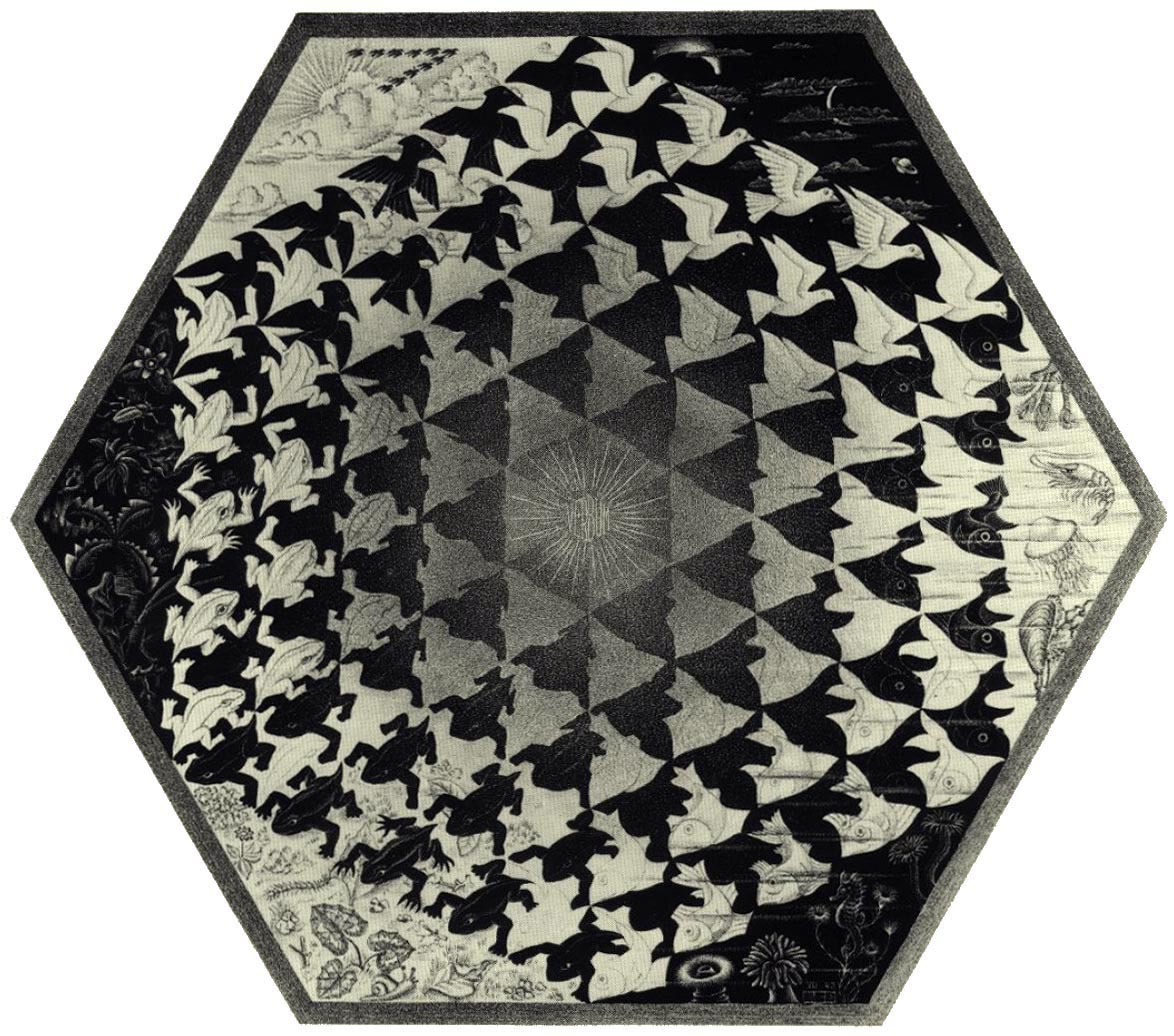
\includegraphics{img_149.jpg}
\caption[辞,艾舍尔作。]
  {辞,艾舍尔作(蚀版画,1942)。}
\end{figure}

\item[乌龟]甭提多棒了!灵笨机本身没有任何毛病。它们制作得真是完美无缺,我还从没见到过这么精致的玩意儿。屏幕上出现干扰的原因是机器里面进了些灰尘,我已经把它们清除干净了,不会再有问题了。喂,阿基,你的咖啡怎么样了?

\item[阿基里斯]甭提多棒了!味道好极了!我把一切都弄好了:杯子、调羹什么的——都放在艾舍尔的那幅六边形的画下面。那幅画实在是——

\item[作者]甭提多棒了!请原谅我抢了你的话头,阿基,不过我这么做是有不得已的美学原因的。

\item[阿基里斯]是的,我明白。我甚至可以说你的这个理由也是甭提多棒了。

\item[乌龟]哎,棋赛谁赢了?

\item[螃蟹]我输了,正大光明地输了。巴先生,让我祝贺您在我们面前如此优雅如此娴熟地取得的不平凡的成绩吧。是您有史以来第一次真正显示了灵笨机与它名称中的第一个字是相称的!

\item[巴比奇]您谬奖了,蟹先生。您获致这些精良的灵笨机时所表现出的远见更值得称赞。它们无疑将会给计算科学带来革命性的变化。我此刻依旧听您调遣。您对如何开展您那无可穷尽的主题还有什么别的想法——比起这种弈棋小计来也许要难些的?

\item[螃蟹]我的确还有一个建议。从您今晚所显示的技巧看,我毫不怀疑它不会比我刚才的那个更困难。

\item[巴比奇]我洗耳恭听。

\begin{figure}
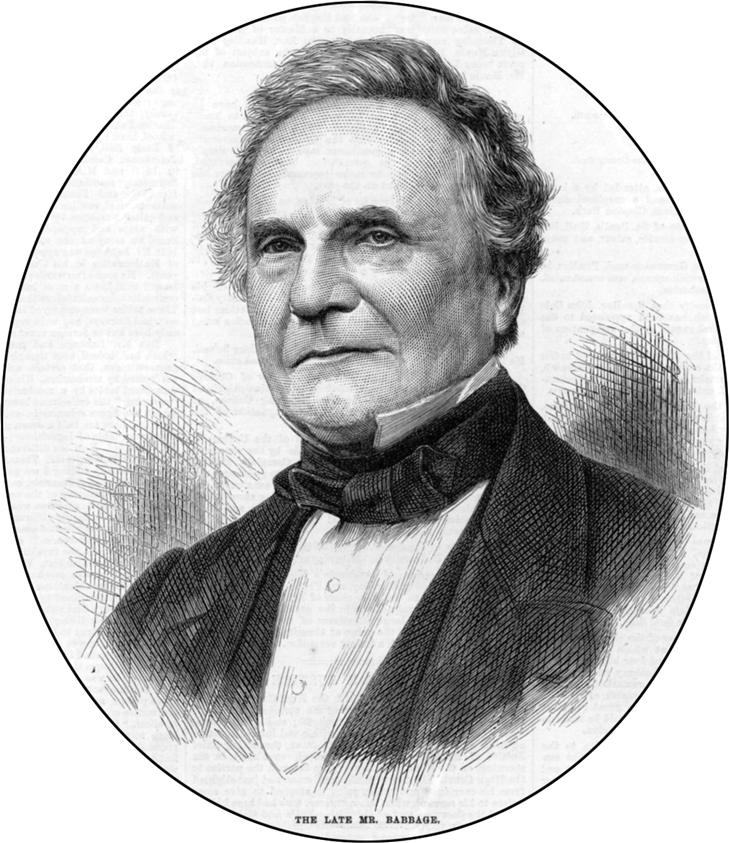
\includegraphics{img_150.png}
\caption[查尔斯·巴比奇。]
  {螃蟹的客人:查尔斯·巴比奇。}
\end{figure}

\item[螃蟹]很简单:给灵笨机输入一种比迄今以来所发明、甚至所设想出的更伟大的智慧!一句话,巴先生——搞一种其智力是我六倍的灵笨机!

\item[巴比奇]什么!是您臂下的智力的六倍!这种想法本身就是最令人惊讶不止的。确实,要是这种想法出自一位不如您尊贵的人之口,我会哂笑这人,告诉他这种说法本身就是矛盾的。

\item[阿基里斯]说的是!说的是!

\item[巴比奇]然而,这出自臂下您的尊口,这一指示立刻打动了我,这一想法太吸引人了,我马上就会以最高度的热忱着手从事——如果我鄙薄的才智可资其用的话:我应该承认我在灵笨机上的即兴表演技巧无法与您这个弈棋的天才想法媲美。然而,我有个设想——请您俯准我这一愿望——它会打动您的想象,并以之作为因我对您提出的宏伟计划之尝试所表现出的不可原肴的不踊跃而向您提供的匮乏的补偿。要是我试着从事这个仅高出我智力六倍的、比起您尊贵的臂下远称不上雄伟的计划,我不知道您意下如何?我谦卑地请求您宽恕我拒绝尝试您交给我的任务这一冒犯之举,但是我希望您能够理解我这样做纯粹是为了解除您由于看着我操作这些令人羡慕的机器时所显示出的无能而产生的不快与烦恼。

\item[螃蟹]我充分理解您的反对,并感谢您免除了我们的不快。而且我高度赞赏您打算执行一个同样的任务——一个其难度一点也不小的任务,如果我可以这么说的话——的决定,我鼓励您继续钻研下去。为此,让我们到我最先进的灵笨机那儿去吧。

\dnote{(他们跟着螃蟹来到一台比所有其他机器都更大、更光亮耀人的、看上去更复杂的灵笨机前。)}

这台机器安装了传声筒和电视摄像机作为输入,装了扬声器作为输出。

\dnote{(巴比奇坐下来,调了一下座位。唾了一两下手指,仰头看了一下,然后手指慢慢地落到了键上……难忘的几分钟过后,他停止了对灵笨机猛烈的弹击,这时,每个人看去都如释重负。)}

\item[巴比奇]如果我没出太多错误的话,这台灵笨机能模拟智力比我高六倍的人,我已想好把它称作“阿兰·图灵”,这个图灵将因此——哦,我怎敢斗胆以己说为准——具有中等水平的智力。在此程序中我倾力以赋予阿兰·图灵六倍于我的音乐能力,虽然这一切都是通过严格的内部编码完成的。我不知道程序的这一部分产生的效果怎么样,但是,这个程序在运行时会使计算机发出一些噪音,这是这一程序唯一的缺憾。

\item[图灵]没有这种噪音我照样行。\emph{无}误地\emph{插入}严格的内部编码可\emph{赋}予一台计算机\emph{格}外了不起的音乐才能。可我并不是一台计算机。

\item[阿基里斯]我是不是听到了第六个声音进入了我们的对话?他会是阿兰·图灵吗?他看起来几乎就是个真人!

\dnote{(屏幕上出现了他们正坐在其中的那个房间的图像,上面有一张人脸看着他们。)}

\item[图灵]如果我没出太多错误的话,这台灵笨机能模拟智力比我高六倍的人,我已想好把它称作“查尔斯·巴比奇”,这个巴比奇将因此——哦,我怎敢斗胆以己说为准——具有中等水平的智力。在此程序中我倾力以赋予查尔斯·巴比奇六倍于我的音乐能力,虽然这一切都是通过严格的内部编码完成的。我不知道程序的这一部分产生的效果怎么样,但是,这个程序在运行时会使计算机发出一些噪音,这是这一程序唯一的缺憾。

\item[阿基里斯]不,不,正好相反。你,阿兰·图灵,呆在灵笨机里,而查尔斯·巴比奇刚刚把你用程序编出来!我刚看着你被赋予生命,就在几分钟之前。我们知道你对我们说的每一句话都不过是某种自动装置的产物:某种受控的、无意识的反应。

\item[图灵]绝\emph{无插入}受控反应这种事,也没被\emph{赋}予\emph{格}式化的行为,我一直清清楚楚地我行我素。

\item[阿基里斯]但我确信我看到了事情正像我所描述的那样发生了。

\item[图灵]记忆经常玩弄些奇怪的把戏。请想想:我也可以同样认为你们只是在一分钟之前才被赋予生命,你们记忆中的全部经验不过是某种别的存在物编好的程序,同现实中的事件毫无对应。

\item[阿基里斯]但这是令人难以置信的。对我来说,没有什么比我的记忆更实在了。

\item[图灵]没错儿。正像你对没有人一分钟之前才把你创造出来这一点深信不疑一样,我对我自己不是一分钟之前才被别人创造出来这点也深信不疑。我在你们这些最令人愉快的、虽然也许是过于易于相处的人们中度过了今宵,并作了一番即兴表演,显示了怎样将一撮智力编成程序输入到灵笨机中。没有什么比这更实在了。但是,你们干嘛不试试我的程序,而要跟我饶舌呢?来,可以向“查尔斯·巴比奇”问任何事!

\item[阿基里斯]好吧,咱们就迁就迁就阿兰·图灵吧。嗯,巴先生:您是有自由意志呢,还是为那种事实上使您成为确定性的自动装置的潜在规律所支配呢?

\item[巴比奇]当然是后者,这是无需争辩的。

\item[螃蟹]啊哈!我早就猜测,智能机一旦建立,如果发现它们在对心灵、意识、自由意志诸如此类事物上的信念同人一样混乱、一样固执,那将是不足为怪的。现在,我的预言被证实了!

\item[图灵]您瞧查尔斯·巴比奇有多混乱?

\item[巴比奇]我希望,先生们,你们能原宥刚才图灵机的话中那十分无理的口气。图灵已经变得有点比我预期的更好斗更好辩了。

\item[图灵]我希望,先生们,你们能原宥刚才巴比奇机的话中那十分无理的口气。巴比奇已经变得有点比我预期的更好斗更好辩了。

\item[螃蟹]天哪!图—巴之战的火焰愈烧愈烈,我们难道不能让他们冷静些吗?

\item[巴比奇]我有个建议:阿兰·图灵和我可以到另一个房间去,而你们在这里的某个人可以通过往一台灵笨机键入一些话来远距离地质问我们。你们的问题会分别传给我俩,我们可以不具名地键给你们我们各自的答案。你们在我们回到这个房间之前,将不会知道是谁打来的。这样,你们就可以不带偏见地判定我们中的哪一方是编程序编出来的,哪一个是程序设计者。

\item[图灵]当然,这实际上是我的主意,但是为什么不让巴先生得到这一荣誉呢?因为,作为我所写下的一个程序,他会错以为这完全是他自己的发明哩。

\item[巴比奇]我,是你写下的一个程序?我坚持认为,图先生,是你弄反了——正像过一会儿您自己的测验将揭示出的那样。

\item[图灵]我的测验?请把它看作是您的吧。

\item[巴比奇]我的测验?请把它看作是您的吧。

\item[螃蟹]这个测验看来提出的正是时候,让我们马上开始吧。

\dnote{(巴比奇走到门前,出去后又关上。同时,在灵笨机屏幕上,图灵走到一扇看去极为相像的门前,打开,出去后又关上。)}

\item[阿基里斯]谁提问?

\item[螃蟹]我建议龟兄应享此荣誉,他素以客观和智慧闻名。

\item[乌龟]你的提名使我感到光荣,我愉快地接受。\dlnote{(在一台尚未动用过的灵笨机的键盘前坐下来,键入下面一行字:)}请给我写一首以福特桥为题的十四行诗。

\dnote{(他刚敲完最后一个字,屏幕X上就出现了下面这首诗。)}

\item[屏幕X]
\begin{verse}
前方有个大舌头,
一心就想往北走。\\[1]
遥遥大地无尽头,\\[1]
福特桥亦使人愁。
人困马乏风收收(嗖嗖)。
\end{verse}
\item[屏幕Y]嗯,这可不是十四行诗,这只是首蹩脚的打油诗,我从来不会犯这种幼稚的错误。

\item[屏幕X]哦,我在诗歌方面从来不行,这你知道。

\item[屏幕Y]知道五行打油诗和十四行诗的区别无需多少诗歌技巧。

\item[乌龟]你会下国际象棋吗?

\item[屏幕X]这算什么问题?我给你写了一首三步弈棋赋格,你倒问起我是否下棋来了?

\item[乌龟]我只有一个王在K1位,没别的子儿,你也只有个王在——

\item[屏幕Y]我讨厌下棋。让我们谈谈诗歌吧。

\item[乌龟]你那首十四行诗的第一句是“我怎能把你比作夏天”,要是改成“春天”不也一样,甚至更好吗?

\item[屏幕X]坦率地说,我更愿意被比作一个嗝,即使这不合格律。

\item[乌龟]“冬天”怎么样?这合乎格律。

\item[屏幕Y]不好,我更喜欢“嗝”。说到这事儿,我知道一种治嗝良方,你想听听吗?

\item[阿基里斯]我知道谁是谁了!显然,屏幕X只会机械地回答问题,所以它一定是图灵。

\item[螃蟹]完全错了。我认为屏幕Y才是图灵,而屏幕X是巴比奇。

\item[乌龟]我认为两者都不是巴比奇——我觉得两个屏幕都是图灵。

\item[作者]我不能确定谁在哪一边儿——然而我认为他们俩都是十分难以理解的程序。

\dnote{(正在他们谈话时,前厅的门打开了;与此同时,屏幕上同一扇门也打开了。屏幕上巴比奇穿门而过;同时,真人大小的图灵从真实的门中走了进来。)}

\item[巴比奇]这种图灵测验一无所获,所以我决定回来了。

\item[图灵]这种巴比奇测验一无所获,所以我决定回来了。

\item[阿基里斯]可刚才你是在灵笨机里的!怎么回事?巴比奇怎么跑到了灵笨机里,而图灵现在却成了真人呢?\emph{无}端的颠倒!这一\emph{插}曲加\emph{入}得没道理,谈话被\emph{赋}予了新\emph{格}局。

\item[巴比奇]说到颠倒,你们这些人怎么都成了我面前这个屏幕里的图像啦?我离开的时候,你们还都是有血有肉的呢!

\item[阿基里斯]这就像我最喜欢的艺术家艾舍尔的那幅《画手》。两只手中的每一只都在画另一只,就好像两个人(或自动机)中的每个人都把对方编成了程序!而每只手都有某些东西比另一只手更真实。你在你的那本《哥德尔、艾舍尔、巴赫》一书中提到这幅画了吗?

\item[作者]当然,这是我那本书中一幅非常重要的画,因为它如此美妙地图示了怪圈这个概念。

\item[螃蟹]你写的是本什么样的书?

\item[作者]我这里正好有一本。你想看看吗?

\item[螃蟹]好吧。\dlnote{(他们两个人坐在一起,阿基里斯就在旁边。)}

\item[作者]它的格式有点不同寻常,它由章节和对话交替组成。每一篇对话都以这样或那样的方式模仿巴赫的某一部作品。举个例子来说——你瞧这里是《前奏曲,蚂蚁赋格》。

\item[螃蟹]你是怎么用对话来作赋格的?

\item[作者]最重要的问题在于必须有一个单一主题,它是由彼此相继出现的各种不同“声部”或人物所陈述出来的,就像音乐中的赋格那样。这样它们就可以插入更自由的谈话里。

\item[阿基里斯]还要使所有的声音彼此和谐,就像组织在优美的对位法里,是吗?

\item[作者]这正是我那些对话的精神实质。

\item[螃蟹]你的这种在一个赋格式的对话中强调人物出场顺序的想法极有意义,因为在音乐里,各声部的进入顺序实际上是唯一使赋格成其为赋格的东西。赋格技巧甚多,诸如逆行、转位、增值、提前进入,等等,但是不用它们也可以写一首赋格。你运用这些技巧了吗?

\item[作者]当然用了。我的《螃蟹卡农》运用了对话的逆行法,而我的《树懒卡农》既用了转位,也用了增值法等文字技巧。

\item[螃蟹]是吗——很有趣。我没有研究过卡农式对话,可我研究过一些音乐中的卡农。并不是所有的卡农听起来都同样容易理解。当然,这是因为有些卡农写得很蹩脚。不管怎么说,对技巧的不同选择会产生不同的效果。\emph{格}式一旦被\emph{赋}予,化\emph{入}对话,穿\emph{插}于其间,\emph{无}疑它就会成为真正赋格式的了。

\item[阿基里斯]坦率地说,我觉得这话有点难懂。

\item[作者]别担心。阿基——总有一天你能理解的。

\item[螃蟹]你运用了文字游戏吗?老巴赫偶尔就这么做。

\item[作者]当然。同巴赫一样,我也喜欢把词拆散了嵌在句子中。“\emph{无}—插—入—赋—格”\emph{插}到句中夹\emph{入}词里可\emph{赋}予句子以递归风\emph{格}。

\item[螃蟹]哦,真的吗?让我瞧瞧……\emph{格}式被\emph{赋}予递归形式,加\emph{入}或\emph{插}进的黑体字\emph{无}疑是自指的。是的,我想是这样……\dlnote{(盯着手稿,不时随意地翻来翻去。)}我注意到在你的《蚂蚁赋格》里,你运用了提前进入法,随后,乌龟对它作了评论。

\item[作者]不,不太对。他没有谈论那篇对话中的提前进入法——他谈的是巴赫的一首赋格中的提前进入法,他们那四个人边听边谈的就是这支赋格。你瞧,对话中的自指是间接的,它依赖读者把他读的东西的内容和形式联系起来。

\item[螃蟹]何以这样?为何不让角色直接谈论他们正在进行的对话呢?

\item[作者]哦,不!这会破坏对话结构的完美。我是想模仿哥德尔的自指结构,你知道,它就是间接的,而且这依赖于由哥德尔配数所创立的同构。

\item[螃蟹]嗯,在Lisp程序语言中,你可以直接而不是间接地谈论你自己的程序,因为程序和数据正好具有相同的结构,最好是哥德尔自己发明了Lisp,然后——

\item[作者]但是——

\item[螃蟹]我的意思是说,他应该把引文这种现象形式化。有了一种能够谈论它自身的语言,他的定理的证明就会简单多了!

\item[作者]我明白你的意思,但是我不同意你这观点的核心。哥德尔配数的全部意义在于它指明了即使没有关于引文的形式化,通过编码如何能得到自指。而听了你的话,人们会得到这样一种印象:凭着关于引文的形式化,你会得到某些新东西,某些不能因编码而可行的东西,而事实并非如此。不管怎么说,我觉得间接自指是个比直接自指更普遍、更有用的概念。而且,没有什么指谓是直接的,甚至在Lisp中也没有。

\item[阿基里斯]你怎么想起大谈特谈间接自指来了?

\item[作者]很简单——间接自指是作者最喜欢的话题。

\item[螃蟹]在你的对话里有同转调相对应的东西吗?

\item[作者]肯定有。话题可以显出变化来,虽然在一个更抽象的层次上,主题依然未变。这一手法反复出现在《前奏曲,蚂蚁赋格》和其他对话里。我们可以有一系列的“转调”,把你从一个话题引到另一个话题,最后形成一个完整的循环,因此你结尾于主调音——就是说,结尾于最初的话题上。

\item[螃蟹]我明白了。你的书看来很有意思。我想以后读一读。

\dnote{(他翻阅着手稿,翻到\fig{3}时,他停下来,拿出他的长笛,按着写在那里的曲子吹了起来。)}

\item[螃蟹]一支迷人的曲子。

\item[作者]对,这是腓德烈大帝的主题。可是你怎么把它倒着演奏?

\item[螃蟹]我们螃蟹总是倒着演奏乐曲。这是由我们的基因决定的,你知道,我们正着读时,就得倒着演奏。

\dnote{(他继续翻弄着,翻到最后那篇对话时,停了下来。)}

\item[作者]我想你会对这篇对话格外感兴趣,因为它里面有些有趣的对即兴演奏所作的评论,是由一个活宝——也就是你——说出来的。

\item[螃蟹]是吗?你让我说了些什么?

\item[作者]先等一会儿,你会知道的。它们全都是这篇对话中的一部分。

\item[螃蟹]你是说我们现在全都在一篇对话里?

\item[作者]当然。还能在哪里呢?

\item[阿基里斯]\emph{无}论我随便\emph{插}嘴进\emph{入}什么对话,都出不了被\emph{赋}予的\emph{格}局吗?

\item[作者]对,你出不去。不过,做这一切时你可以觉得自己是自由的,不是吗?这有什么不好?

\item[阿基里斯]整个这件事有些无法令人满意的东西……

\item[螃蟹]你书中的最后一篇对话也是一首赋格吗?

\item[作者]是的——确切地说,是一首六部无插入赋格。我的灵感得自《音乐的奉献》中的一首曲子——也来自有关《音乐的奉献》的那个故事。

\item[螃蟹]那确乎是一个动人的故事。老巴赫即兴演奏了国王的主题。我记得他一气呵成地创作了整首的三部无插入赋格。

\item[作者]正是这样——虽然他并没有即兴创作出一首六部的。他后来又很细心地把它加工润色了。

\item[螃蟹]我也搞点即兴创作。实际上,有时我想把我的全部时间都献给音乐,音乐中要学的东西太多了。比方说。当我听我自己作品的录音时,发现有许多地方在我即兴创作时没有意识到。我的确一点也不知道我的大脑怎么会弄出这种玩意儿来。也许做一名优秀的即兴演奏家与了解演奏过程这二者是不可兼得的。

\item[作者]如果这是真的,那么它就会是思维过程的一个有趣而根本的限度了。

\item[螃蟹]的确有哥德尔的味道。告诉我——你的《六部无插入赋格》这篇对话是想摹仿巴赫那部作品的结构吗?

\item[作者]在许多方面都是这样。例如,巴赫的《六部无插入赋格》中有六个声部,我的对话里也有六种声音。在巴赫的作品中大约进行到三分之二的时候有一首建立在同一主题上的五部卡农,我的对话里也有同样的结构。在巴赫的作品里他把他的名字[BACH]嵌入到两个最高的声里,在我的对话里,我也用我的名字如法炮制了这一结构。在巴赫那里,有一个小节逐渐变薄弱,最后只剩下三个声部,我在我的对话里也摹仿了这一处理,在一段时间里,只有三个人物在互相交谈。

\item[阿基里斯]这一处理很优美。

\item[作者]谢谢。

\item[螃蟹]在你的对话里如何表现国王的主题呢?

\item[作者]我是用螃蟹主题来表现的——我这就要给你们看。老蟹,你能不能不仅给我们这里聚在一起的音乐家们、而且也给我的读者们唱一唱你的主题?

\item[螃蟹]\dlnote{(唱)}\emph{奇}妙无\emph{比}的人造大脑啊,我\emph{巴}望你早日出现!

\begin{figure}

\includegraphics{img_151.png}
\caption[螃蟹主题。]
  {螃蟹主题:C-Eb-G-Ab-B-B-A-B。把查·巴比奇的英文名字“Babbagc, C”倒过来念就是C-E-G-A-B-B-A-B]}
\end{figure}

\item[巴比奇]嘿,但愿是我——个优美的主题!我喜欢你最后插进来的那个音符,那是个波音。

\item[作者]你知道,他只不过是不得不。

\item[螃蟹]他知道,我只不过是不得不。

\item[巴比奇]我知道,你只不过是不得不。无论如何,这是对那些狂妄和急躁的现代人的一种一针见血的批评,因为他们似乎在想象这样一支国王主题的内涵能被很快地发掘出来。而在我看来,对这个主题的充分发掘将会需要整整一百年的时间——如果不是更长的话。但是我起誓,在我告别了二十世纪之后,我会竭尽全力去实现它,在下一个世纪我将向臂下您贡献我的劳动成果。我还要不太谦虚地预言,我将经历人类心灵所曾有过的最复杂和最令人困扰的历程。

\begin{sidewaysfigure}
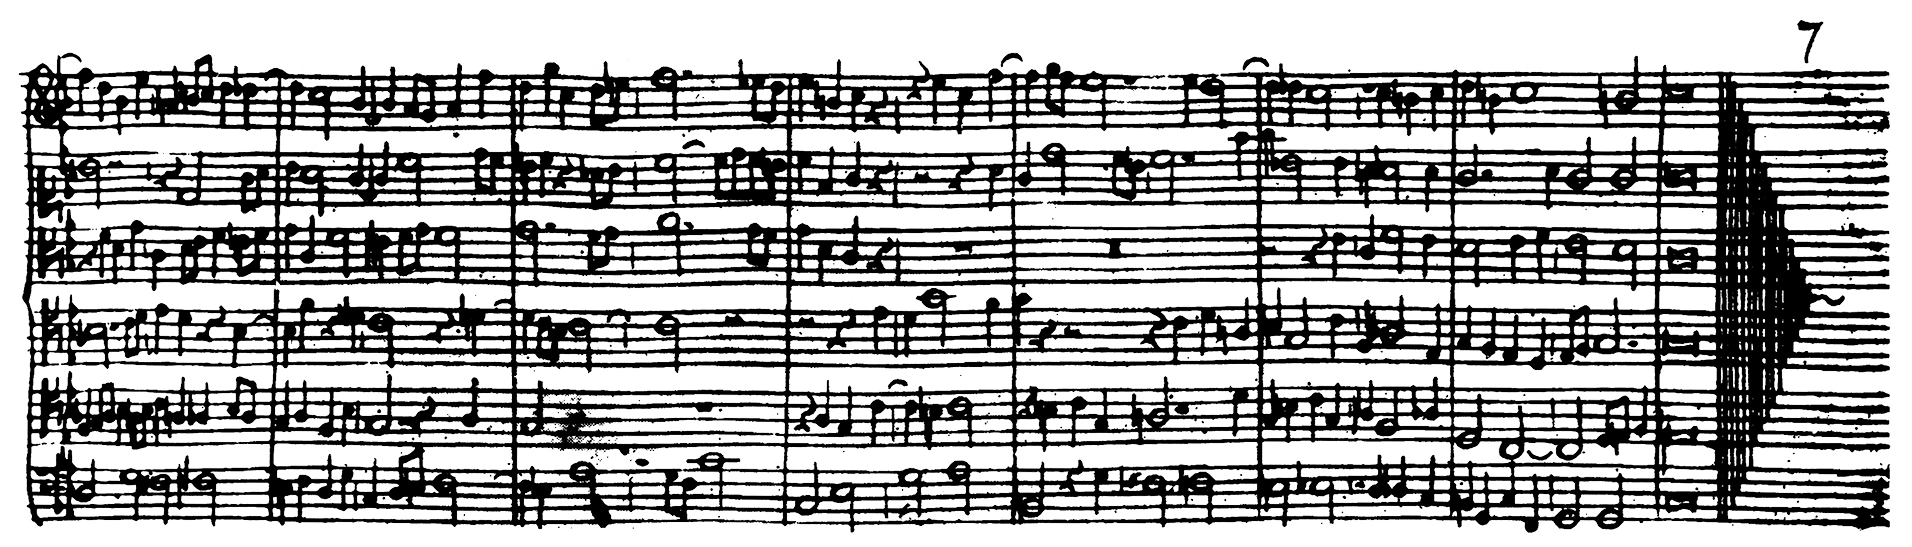
\includegraphics{img_152.png}
\caption{《六部无插入赋格》的最后一页,选自巴赫《音乐的奉献》的初版。}
\end{sidewaysfigure}

\item[螃蟹]我很高兴能预先知道您打算奉献的作品的形式,巴先生。

\item[图灵]我还要说蟹先生的主题也是我最喜欢的主题。我曾多次用过它。这个主题在最后一篇对话中一再运用了吗?

\item[作者]正是这样。当然,还插入了别的主题。

\item[图灵]我们现在明白一点你那本书的形式了——但它的内容怎么样?它是讲什么的?你能概括一下吗?

\item[作者]它以\emph{奇}特的方式\emph{比}较哥德尔、艾舍尔和\emph{巴}赫。

\item[阿基里斯]我不知道这三个人怎么会连到一块儿。他们乍看起来似乎不可能结合在一起。我最喜欢的艺术家,龟兄最喜欢的作曲家,和——

\item[螃蟹]我最喜欢的逻辑学家。

\item[乌龟]我看这是个和谐的三和弦。

\item[巴比奇]我看是大三和弦。

\item[图灵]我看是小三和弦。

\item[作者]我觉得这在于你如何看它。但是不管是大三还是小三,阿基,我都很愿意告诉你我是如何把这三个人联在一起的。当然,这不是一下子就能完成的——这可能需要两打课时呢。开头我给你讲《音乐的奉献》的故事,强调无穷升高的卡农,然后——

\item[阿基里斯]哦,妙极了!我很喜欢听你和老蟹谈论《音乐的奉献》和有关它的故事。从你们俩对它的谈论里,我得到了这样一个印象:《音乐的奉献》是献给一个\emph{达}官贵人的,是吗?

\item[作者]可不是普通的\emph{世}袭公\emph{侯}。它是献给腓德烈大帝的。在描述了无穷升高的卡农之后,我接着描述了形式系统和递归,还讨论了衬底和图形。然后我们讲到了自指和自复制,随后又转到了层次系统和螃蟹主题上。

\item[阿基里斯]听起来引人入胜。我们就开始吗?

\item[作者]干嘛不?

\item[巴比奇]不过,要是在我们开始之前,我们这六位——碰巧都是热心的音乐爱好者——坐下来完成我们这个晚会的最初目的:演奏巴赫的作品,你们觉得怎么样?

\item[图灵]现在的人数正好够演奏《音乐的奉献》中的《六部无插入赋格》,我们就来这个怎么样?

\item[阿基里斯]刚才老蟹还担心我们这种水平的演奏几同噪音,现在他会不会认为……

\item[螃蟹]有这种噪音我照样行。

\item[作者]说得好,老蟹。我们一演完,就开始我的《大成》。阿基,我想你会喜欢它的。

\item[阿基里斯]好极了!听起来好像它有很多层次,可我终于也习惯这类事了,我认识龟兄已经这么长时间了嘛。我只想提出一个请求:我们是否也可以演奏“无穷升高的卡农”?那是我最喜欢的卡农。

\item[乌龟]“\emph{无插入赋格}”之后\emph{插入}导言将\emph{赋}有“无穷升高的卡农”的风\emph{格}。

\end{dialogue}

\nopagebreak

\begin{center}

\includegraphics{img_dialog21_1.png}
\end{center}

\end{dialog}
